%!TEX root = proj_report_outline.tex
\chapter{Evaluation}
Following the completed implementation and infrastructure setup an evaluation of the project was carried out on prototype. The evaluation was designed primarily to verify whether or not the prototype developed was successful in fulfilling the requirements identified as in scope in Section \ref{S:evaluationScope}.

\section{Test \rom{1} - Collaboration Functionality Fulfilment}

\subsection{Motivation}
PitchHub's primary goal is to facilitate collaboration within the innovation community. To do this PitchHub seeks to engage all roles in the innovation community by focusing de-constructing ideas to appeal their expertise - in terms of  value proposition, business opportunity, challenges, and solution. Test \rom{1} seeks to verify that the prototype supports the behaviour necessary to facilitate this collaboration. As discussed in Section \ref{C:requirements} this behaviour is distilled in the requirements D1, D2.1 and D2.2.

\subsection{Results}
The user stories which affirm the fulfilment of requirements D1, D2.1 and D2.2 in \textit{TB1} confirm support of the following behaviour:

\paragraph{Requirement D1's user stories specify the ability to:} post Pitch Cards, make suggestions on Pitch Points, accept/reject suggestions, comment on Pitch Points, comment on suggestions and mark Pitch Cards as completed/active.

\paragraph{Requirement D2.1's user stories specify the ability to:} scope entities such as Pitch Cards, suggestions, and one's identity such that unintended viewers are avoided. To ensure the completeness of these user stories, each scope/viewer level combination is tested. These combinations are displayed in Fig \ref{fig:architecturescope_matrix_evaluation}.

\begin{figure}[ht]
    \centering
    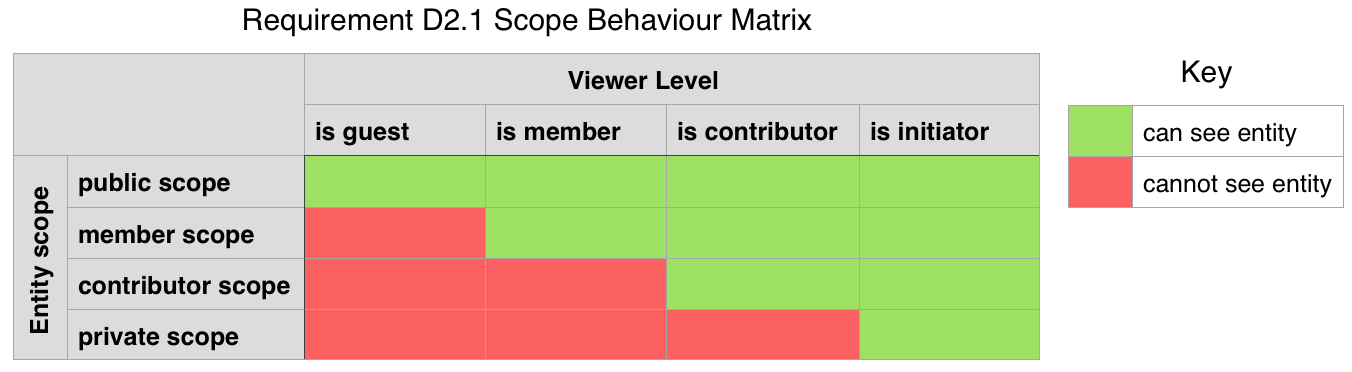
\includegraphics[width=1\textwidth]{scope_matrix}
    \caption{The scope matrix which illustrates the relationship between viewer level and entity scope in regards to viewing the entity.}
    \label{fig:architecturescope_matrix_evaluation}
\end{figure}

\paragraph{Requirement D1's user stories specify that:} users who have viewed a Pitch Card are able to be seen as a ``viewer'' by the PitchCard's initiator.

\subsection{Discussion}
The design of this experiment was guided by two main questions: first, ``what behaviours are needed to facilitate collaboration in the innovation community?'' And second, ``how can these behaviours be verified as functional from a user's point of view?''. In regards to the first question, determining what behaviours were required was to an extent already completed by Callaghan Innovation through their conceptualisation of PitchHub. To formalise these behaviours Callaghan Innovation and I collaborated on the specification of the user stories.
In regards to the second question, realistically simulating user interaction was identified as key. Manually testing the various behaviours and scope combinations would be time-consuming and tedious. \textit{TB1} automates this simulation with the added benefit of assertions, making it easy to verify that expected behaviour is indeed satisfied.
Concluding on the fulfilment of requirements D1, D2.1 and D2.2 largely relies on whether the behaviours specified in relation to the first question accurately reflects the behaviour required by the innovation community. Generalising what a large population needs is a difficult task but it is my belief that because the user stories tested were created in collaboration with Callaghan Innovation, who is a large participant in the innovation community, they are therefore meet the level of credibility required for the purposes of this test. As such, it is concluded that requirements D1, D2.1 and D2.2 have been fulfilled.

\section{Test \rom{2} - Deployed Prototype Analysis}\label{S:test_2}
At the time of writing, the prototype, \textit{TB3}, has been successfully been released to Callaghan Innovation and is ready for use. Unfortunately use of the prototype by Callaghan Innovation has not yet fully commenced. Without substantial activity to analyse this test was unable to be completed. It is expected that the access code will be distributed by the Callaghan Innovation stakeholders to the wider organisation in the coming weeks.

\section{Test \rom{3} - Community Size Support}

\subsection{Motivation}
Supporting collaboration within the innovation community firstly requires that sheer size of the community is able to be supported. Test \rom{3} seeks to test whether the PitchHub prototype could support the entire NZ innovation community. The sizes tested against are derived from the Statistics NZ data, where the expected size is estimated to be a population of 400,000 and the worst case size is estimated to be a population of 600,000.

Test \rom{3} uses the prototype on \textit{TB2} in a diverse ``3, 4'' secret sharing scheme configuration (2x MongoDB replica sets and 2x Postgres instances).

\subsection{Results}

\begin{figure}[ht]
    \centering
    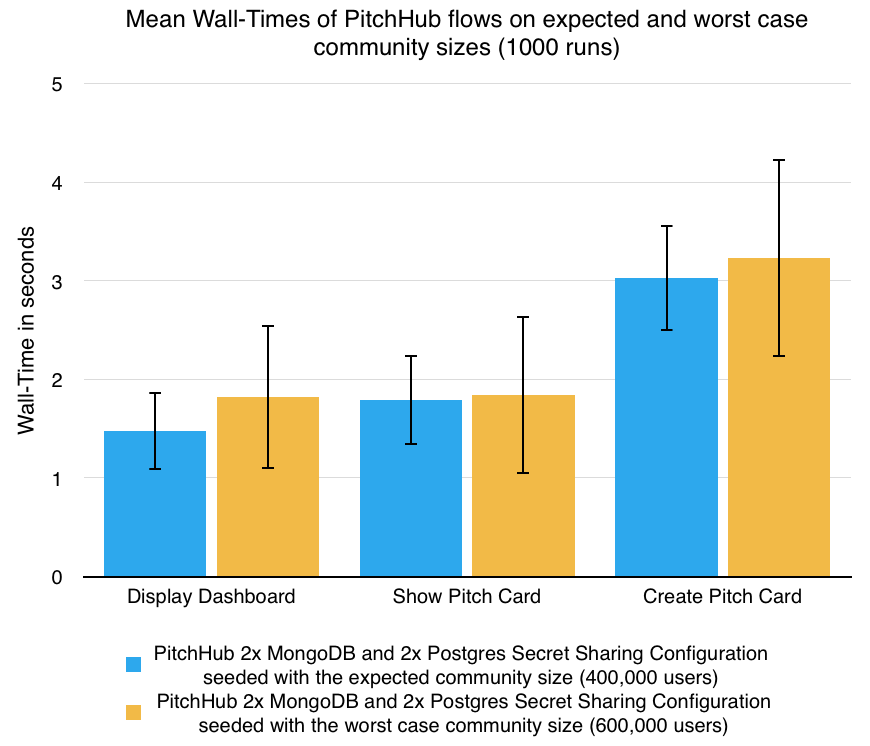
\includegraphics[width=1\textwidth]{experiment_3_results}
    \caption{The mean response times with standard deviation for PitchHub flows: display dashboard, show Pitch Card, and create Pitch Card, under both expected and worst case community sizes. There is a very negligible performance difference between the two community sizes. Each size elicits mean response times that fall under Nielsen's third threshold. }
    \label{fig:test_3_results}
\end{figure}

\subsection{Discussion}

Fig \ref{fig:test_3_results} illustrates that the PitchHub prototype in a 2x MongoDB and 2x Postgres Secret Sharing configuration can support the innovation community at both the expected and worst case sizes (derived from the Statistics NZ data in Table \ref{tab:title}). In terms of Nielsen's response thresholds, each flow falls under Nielsen's third threshold (1 =\textless 10 seconds): where a users attention is still maintained but the wait-time interrupts flow of thought. Given that each flow in both community sizes meets the acceptable response threshold it can be concluded that the prototype satisfies requirement D4.

The difference in community sizes shows only a negligible performance difference in mean wall-time for each flow. This is because, even at the worst-case size, the database is only medium in size - where the entire database is storing between 10\textsuperscript{5} and 10\textsuperscript{7} records and can still fit on a single server \cite{Large8:online}. At this size, performance is not effected by amount of data stored. For performance to be affected by database size, the user size would need to climb to XXX,XXX or the contribution distribution would need to shift to the right.

\section{Test \rom{4} - Overhead of Threshold Scheme Security}

\subsection{Motivation}
The secret sharing service is an important part of keeping sensitive user data secure. A consequence of this service is a loss of performance - primarily a consequence of the latency introduced by the queries to the \textit{n} secret keepers and added processing on the application server in reconstructing the secrets. Test \rom{4} seeks to measure the overhead of this service and discuss whether the security afforded is worth the performance loss.

\subsection{Results}

\begin{figure}[ht]
    \centering
    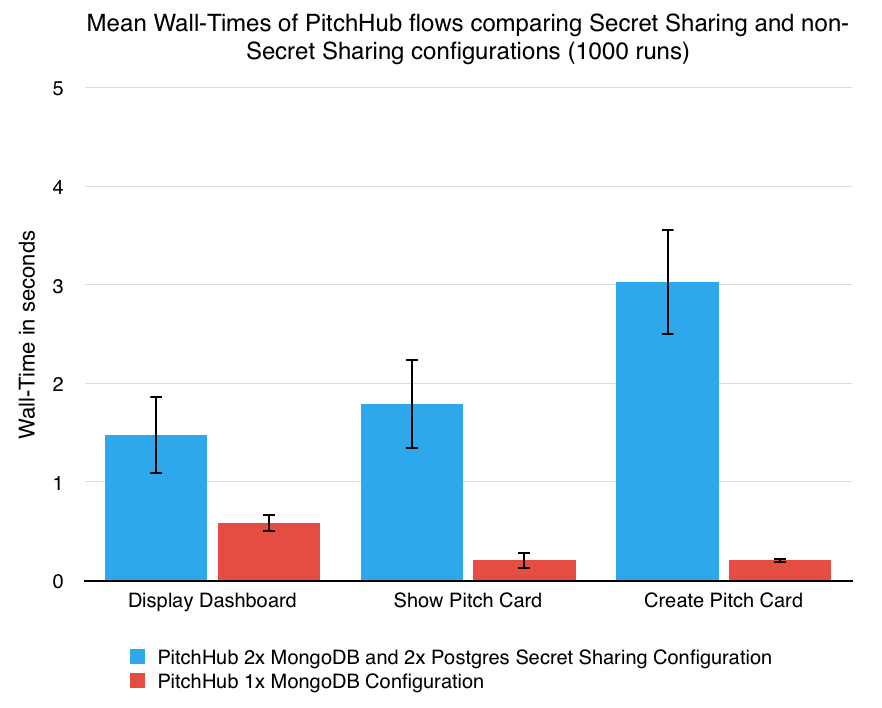
\includegraphics[width=1\textwidth]{experiment_4_results}
    \caption{Comparison of the mean response times with standard deviation for PitchHub flows: display dashboard, show Pitch Card, and create Pitch Card, in both Secret Sharing and non-Secret Sharing configurations. There is a very significant performance difference between the two configurations. The non-Secret Sharing configuration falls under Nielsen's second threshold whereas the Secret Sharing configuration falls under the third. }
    \label{fig:test_4_results}
\end{figure}

\subsection{Discussion}
Fig \ref{fig:test_4_results} illustrates the difference in mean wall-times between Secret Sharing and non-Secret Sharing configurations. It is clear that the Secret Sharing service incurs a significant loss in performance. The most prominent case is the Create Pitch Card flow, where the Secret Sharing configuration is 14x slower. There are a number of important differences between the two configurations that contribute to this loss. The most important of which is operations involved, the Create Pitch Card flow in the non-Secret Sharing configuration is essentially an insert statement followed by a redirect to the newly saved Pitch Card, whereas in the Secret Sharing configuration the Pitch Card object is split into \textit{n} shares, \textit{k-1} of these are adapted to Postgres' ORM format, each share is saved to their respective secret keepers, and on completion of the \textit{n} saves the action is concluded with a redirect to the newly saved Pitch Card. The Secret Sharing configuration is simply doing more and is therefore taking longer.
Determining whether this overhead is acceptable is an inherently subjective task. Strictly in light of Nielsen's thresholds it is not worth it. As the non-Secret Sharing configuration meets the second threshold while the Secret Sharing configuration slips to meet the third. But ultimately, the question that must be asked is: ``Is the noticed delay and interrupted flow of thought worth the security afforded by the Secret Sharing scheme?''. Based on the nature of the data being served I believe that this overhead is indeed worth it. To view the problem from another perspective, it seems reasonable to trade 2 seconds in delay for assured security in the event that secret keepers be breached.

\section{Test \rom{5} - Overhead of Secret Keeper Diversity}

\subsection{Motivation}
To strengthen the security afforded by the secret sharing service diversity was added to the secret keepers. A consequence of this is that the service is now only as fast as it's slowest secret keeper. Test \rom{5} seeks to measure the overhead of this added diversity and discuss whether the extra security afforded is worth the performance loss.

Test \rom{5} uses the prototype on \textit{TB2} in a both a diverse ``3, 4'' secret sharing scheme configuration (2x MongoDB replica sets and 2x Postgres instances) and a homogeneous ``3, 4'' secret sharing scheme configuration (4x MongoDB replica sets).

\subsection{Results}

@KB, figure \ref{fig:test_5_results} should be here...

\begin{figure}[ht]
    \centering
    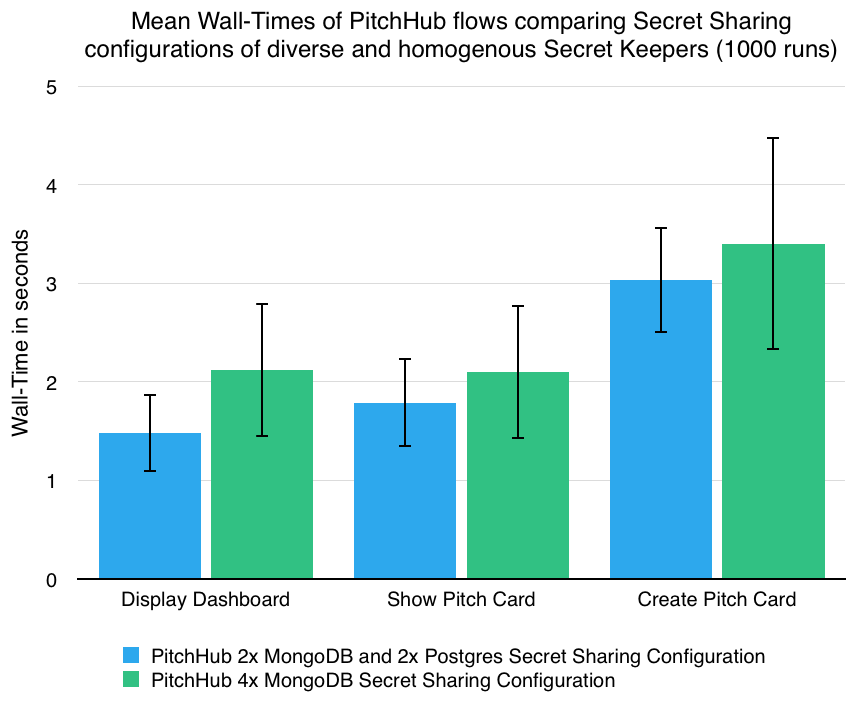
\includegraphics[width=1\textwidth]{experiment_5_results}
    \caption{Comparison of the mean response times with standard deviation for PitchHub flows: display dashboard, show Pitch Card, and create Pitch Card, in both diverse and homogeneous secret keeper configurations. There is a noticeable performance difference between the two configurations where the diverse configuration performs faster. Both configurations fall under Nielsen's third threshold limit.}
    \label{fig:test_5_results}
\end{figure}

\subsection{Discussion}
Fig \ref{fig:test_5_results} illustrates the difference in mean wall-times between Secret Sharing configurations with diverse and homogeneous secret keepers. The diverse configuration is consistently faster than the homogeneous configuration across all flows. The 10\% increase is likely because of the choice of secret keepers used - since MongoDB is less performant than Postgres in both read and write operations \cite{van2012sensor}. 
A disadvantage with the Postgres instances is that they do not provide the same assurance of availability as the MongoDB replica set secret keepers. This may present itself as a problem should the Postgres instance become unavailable resulting in it's shares becoming unavailable and hence harder to meet the required \textit{k} shares needed for reconstruction. 
Overall, these results indicate that this particular diverse configuration is worth the extra implementation effort as it not only solves the Secret Sharing scheme's redundancy issue but also performs better. 

\section{Test \rom{6} - Concurrent Load Support}
\subsection{Motivation}
Beyond being able to satisfy individual requests within an acceptable threshold it is important the PitchHub is able to do this while under the load of the innovation community. Test \rom{6} aims to assess the extent of the load that can be sustained by \textit{TB2} in a 2x MongoDB and 2x Postgres Secret Sharing configuration. This test specifically looks at the load that can be supported by the Show Pitch Card flow as this is assumed to be the most frequently requested flow.

\subsection{Results}

Fig \ref{fig:test_6_results} should be here...

\begin{figure}[ht]
    \centering
    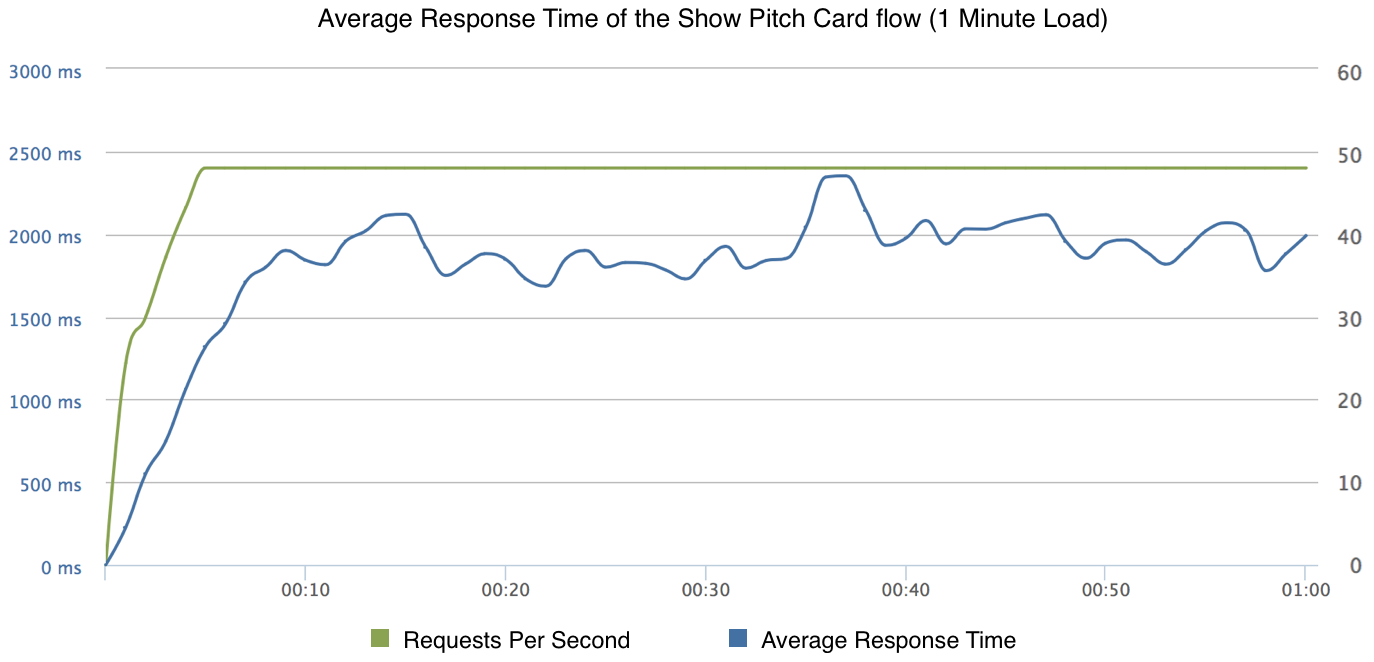
\includegraphics[width=1\textwidth]{experiment_6_results}
    \caption{Load test of the Show Pitch Card flow in a 2x MongoDB and 2x Postgres Secret Sharing configuration. Under 120 requests per seconds the prototype is able to maintain a 2 second response time average. }
    \label{fig:test_6_results}
\end{figure}

\subsection{Discussion}
From the data in Fig \ref{fig:test_6_results}, it is apparent that \textit{TB2} can reliably sustain a load of 50 requests per second while maintaining an average response time of 2 seconds. This is significant as it reveals that the individual response times found in Fig \ref{fig:test_3_results} can be sustained at load. Beyond 50 requests per second \textit{TB2} begins to return error code 500s, meaning that the server knows it has had a problem fulfilling the request.
Determining exactly how many users 50 requests per second may support is difficult to estimate. Frequency analysis on \ref{S:test_2}'s results would have been helpful in identifying the community's usage patterns. Nevertheless, without this data, the following assumptions have been made: the load is distributed evenly, each user uses PitchHub once a day, and each user session is 10 requests deep (page requests). Calculating the necessary requests per second for the expected and worst case community sizes using these assumptions results in the following:

\begin {table}[H]
\begin{center}
\begin{tabular}{ |p{2cm}||p{6cm}| }
 \hline
 Size & Required Requests Per Second (rps)\\
 \hline
    Expected & 45 rps\\
 \hline
    Worst case & 70 rps\\
 \hline
\end{tabular}
\end{center}
\end{table}
Based on these assumptions \textit{TB2} can therefore satisfy the load of the expected community size but not the worst case. To increase the load supported \textit{TB2} could be either scaled vertically or horizontally, such that the application server size is increased or a load balancer and other servers are added. 
One major drawback of the assumptions is that the load is unlikely to be even. Peaks in usage will occur throughout the day and it is this maximum peak load that will need to be satisfied. Once \textit{TB3} has gathered sufficient data, these peaks may be modelled, and subsequently more accurate load estimates can be made.
